% Copyright 2026 Sreeram Anil
% SPDX-License-Identifier: CC-BY-4.0
% =============================================================================
%  The battery cell and its equivalent-circuit model — foundational chapter
% =============================================================================
\chapter{The battery cell and its equivalent-circuit model}
\label{ch:ecm}

Everything in this report is an estimator for one of two plants, and this chapter describes the
first of them together with the model that the estimators are given. The distinction matters:
the plant (\code{include/estkit/battery/plant\_ecm.hpp}) is an enhanced equivalent-circuit cell
with hysteresis, a thermal state and ageing; the estimator model
(\code{include/estkit/battery/ecm\_model.hpp}) is the four-state, lookup-table version that a
production battery-management system (BMS) could actually run on a microcontroller. The
difference between them is not an oversight but the experiment: \cref{sec:ecm-mismatch} lists it
item by item.

The chapter proceeds from physics to code. \cref{sec:ecm-physics,sec:ecm-ocv,sec:ecm-entropy}
establish the thermodynamic quantities --- state of charge, open-circuit voltage, entropic
coefficient --- and derive the full-cell OCV from the electrode potentials of Chen
et~al.~\cite{chen2020parameterization}. \cref{sec:ecm-thevenin,sec:ecm-hyst,sec:ecm-thermal,%
sec:ecm-arrhenius,sec:ecm-aging} build the plant one mechanism at a time, each with the exact
discrete form implemented in the library. \cref{sec:ecm-estimator} gives the estimator model and
its Jacobians in closed form, \cref{sec:ecm-obs} analyses its observability, and
\cref{sec:ecm-params,sec:ecm-mismatch} tabulate the parameters and the deliberate mismatches.

\section{The lithium-ion cell as a dynamical system}
\label{sec:ecm-physics}

A lithium-ion cell stores energy by moving lithium between two intercalation hosts. In the cell
modelled here --- an \SI{5}{\ampere\hour}, 21700-format NMC811/graphite cell with the electrode
data of the LG~M50 \cite{chen2020parameterization} --- lithium leaves the graphite negative
electrode on discharge, crosses the electrolyte as Li$^+$ and intercalates into the
LiNi$_{0.8}$Mn$_{0.1}$Co$_{0.1}$O$_2$ positive electrode, with the compensating electron travelling
through the external circuit. Three consequences define the estimation problem.

\begin{definition}[State of charge]\label{def:ecm-soc}
The state of charge $\soc$ is the fraction of the cell's present usable capacity $Q$
(\si{\ampere\hour}) that remains available, defined by the charge balance
\begin{equation}
\frac{\mathrm{d}\soc}{\mathrm{d}t} = -\frac{\eta(i)\,i(t)}{3600\,Q},
\label{eq:ecm-socdef}
\end{equation}
with $i>0$ on discharge and $\eta(i)$ the coulombic efficiency of \cref{sec:ecm-coulomb}.
\end{definition}

$\soc$ is not measurable. It is defined by an integral of the current, so any current-sensor
error accumulates without bound, and it is a \emph{relative} quantity referred to a capacity $Q$
that itself drifts over the cell's life. The only direct observation is the terminal voltage.

\begin{definition}[Open-circuit voltage]\label{def:ecm-ocv}
The open-circuit voltage $\ocv(\soc,T)$ is the terminal voltage of the cell at zero current after
all concentration gradients have relaxed. It is the difference of the two electrode equilibrium
potentials at the stoichiometries corresponding to $\soc$.
\end{definition}

Because $\ocv$ is a thermodynamic function of the lithium distribution and the lithium
distribution is what $\soc$ measures, the map $\soc\mapsto\ocv$ is the bridge between the
unmeasurable state and the measurable output. \emph{This one function carries the entire
observability of state-of-charge estimation}: in the linearised measurement equation of
\cref{sec:prelim-ocvslope}, the SOC appears through the single scalar
$\partial\ocv/\partial\soc$ and through nothing else. Where that slope is large, a millivolt of
voltage information is worth little SOC error; where it is flat, the same millivolt is worth
percent. Every result in Part~XIII is, at bottom, a consequence of this statement, and
\cref{sec:ecm-obs} makes it quantitative.

The third consequence is that the cell is not a thermodynamic device but a kinetic one: at any
non-zero current the terminal voltage differs from $\ocv$ by an overpotential composed of an
instantaneous ohmic drop, one or more relaxing diffusion/charge-transfer terms, and a
path-dependent hysteresis. The equivalent-circuit model of \cref{sec:ecm-thevenin} is a
lumped, empirical description of exactly those terms.

\section{Electrode potentials and the full-cell OCV}
\label{sec:ecm-ocv}

\subsection{The Chen 2020 electrode potential functions}
The library uses the fitted open-circuit-potential functions of
Chen et~al.~\cite{chen2020parameterization} as distributed in the \texttt{Chen2020} parameter set
of PyBaMM \cite{sulzer2021pybamm}. Let $x = c_{\mathrm{n}}/c_{\max,\mathrm{n}}$ and
$y = c_{\mathrm{p}}/c_{\max,\mathrm{p}}$ be the negative- and positive-electrode
stoichiometries. Then, in volts against Li/Li$^+$,
\begin{align}
U_{\mathrm{n}}(x) &= 1.9793\,e^{-39.3631x} + 0.2482
 - 0.0909\tanh\!\big(29.8538(x-0.1234)\big) \notag\\
 &\quad - 0.04478\tanh\!\big(14.9159(x-0.2769)\big)
       - 0.0205\tanh\!\big(30.4444(x-0.6103)\big),
\label{eq:ecm-Un}\\[1mm]
U_{\mathrm{p}}(y) &= -0.8090\,y + 4.4875
 - 0.0428\tanh\!\big(18.5138(y-0.5542)\big) \notag\\
 &\quad - 17.7326\tanh\!\big(15.7890(y-0.3117)\big)
       + 17.5842\tanh\!\big(15.9308(y-0.3120)\big).
\label{eq:ecm-Up}
\end{align}
The graphite expression \eqref{eq:ecm-Un} reproduces the three staging plateaux of the
lithiated-graphite phase diagram through its three $\tanh$ terms and the steep rise towards
$x\to 0$ through the exponential. The two nearly cancelling $\tanh$ terms in \eqref{eq:ecm-Up}
are a fitting device: their difference produces the finite slope of the NMC811 potential around
$y\approx 0.31$ without introducing a discontinuity. Both functions are differentiable in closed
form, and the library implements $U_{\mathrm{n}}'$, $U_{\mathrm{p}}'$ analytically because the
OCV slope is needed at every sample by every filter.

\subsection{Stoichiometry as a function of SOC: the lithium balance}
The electrode potentials are functions of stoichiometry; the model needs them as functions of
$\soc$. The mapping follows from conservation of lithium.

Let $\varepsilon_k$ be the active-material volume fraction, $L_k$ the coating thickness and $A$
the electrode area of electrode $k\in\{\mathrm{n},\mathrm{p}\}$. The amount of charge
corresponding to a unit change of stoichiometry is
\begin{equation}
q_k = F\,\varepsilon_k L_k A\, c_{\max,k} \quad[\si{\ampere\second}],
\label{eq:ecm-qk}
\end{equation}
with $F = \SI{96485.33}{\coulomb\per\mole}$ the Faraday constant. With the geometry of
\cref{tab:ecm-chen} this gives $q_{\mathrm{n}} = \SI{20979}{\ampere\second} =
\SI{5.83}{\ampere\hour}$ and $q_{\mathrm{p}} = \SI{31436}{\ampere\second} =
\SI{8.73}{\ampere\hour}$: the electrodes are over-sized relative to the \SI{5}{\ampere\hour}
nominal capacity, as they must be in a cell that is neither plated nor over-delithiated at its
voltage limits.

Passing $Q_{\mathrm{nom}} = \SI{5}{\ampere\hour}$ of charge between $\soc=1$ and $\soc=0$
therefore changes the stoichiometries by
\begin{equation}
\Delta x = \frac{3600\,Q_{\mathrm{nom}}}{q_{\mathrm{n}}} = 0.85798, \qquad
\Delta y = \frac{3600\,Q_{\mathrm{nom}}}{q_{\mathrm{p}}} = 0.57259,
\label{eq:ecm-dxdy}
\end{equation}
i.e.\ the graphite is cycled over \SI{85.8}{\percent} and the NMC over \SI{57.3}{\percent} of its
theoretical range. Anchoring at the fully charged state,
\begin{equation}
x(\soc) = x_{100} - (1-\soc)\,\Delta x, \qquad
y(\soc) = y_{100} + (1-\soc)\,\Delta y,
\label{eq:ecm-xyz}
\end{equation}
with $x_{100}=0.9014$ and $y_{100}=0.2700$. These two numbers are \emph{not} independent fits:
they are the initial solid concentrations of the PyBaMM \texttt{Chen2020} parameter set divided
by the respective $c_{\max}$, so that the estkit cell starts from exactly the lithium
distribution a PyBaMM simulation of the same cell would start from. This is what makes the
cross-validation of \cref{ch:spm} a like-for-like comparison. \eqref{eq:ecm-xyz} evaluated at
$\soc=0$ gives $x_0 = 0.04342$ and $y_0 = 0.84259$, both comfortably inside the range over which
\eqref{eq:ecm-Un}--\eqref{eq:ecm-Up} were fitted.

The full-cell equilibrium voltage and its slope follow immediately by the chain rule:
\begin{align}
\ocv(\soc) &= U_{\mathrm{p}}\big(y(\soc)\big) - U_{\mathrm{n}}\big(x(\soc)\big),
\label{eq:ecm-ocv}\\
\frac{\partial\ocv}{\partial\soc}(\soc)
 &= -\Delta y\, U_{\mathrm{p}}'\big(y(\soc)\big) - \Delta x\, U_{\mathrm{n}}'\big(x(\soc)\big).
\label{eq:ecm-docv}
\end{align}
The minus signs are the whole story of an intercalation cell: discharging lowers $y$ towards
$y_0$, along which $U_{\mathrm{p}}$ \emph{falls}, and raises $x$ towards $x_{100}$, along which
$U_{\mathrm{n}}$ \emph{falls} --- so the cell voltage falls twice over.

\begin{figure}[H]\centering
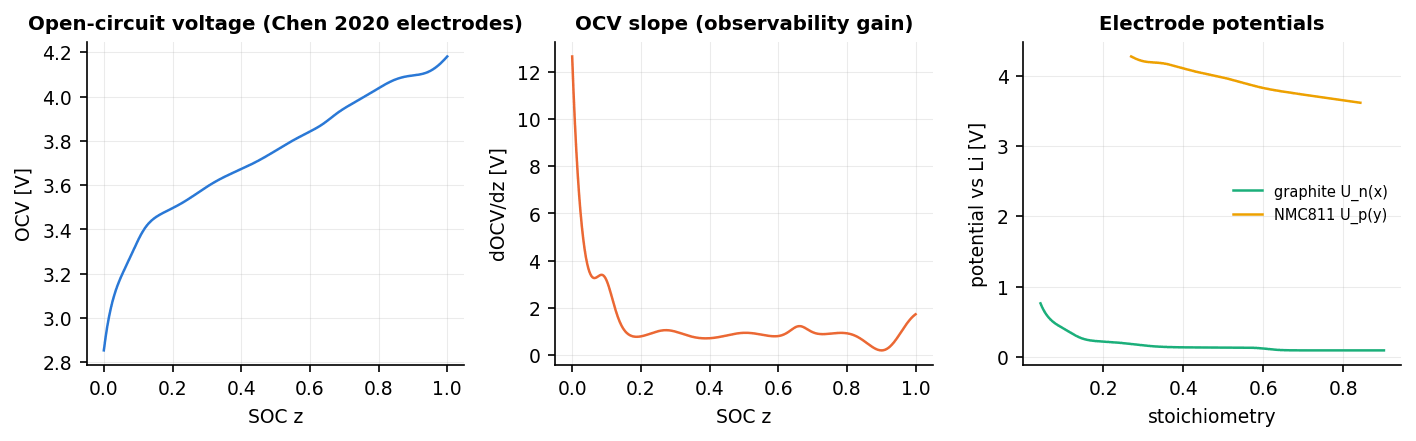
\includegraphics[width=\textwidth]{figures/model_ocv.png}
\caption{The full-cell open-circuit voltage built from the Chen~2020 electrode potentials.
Left: $\ocv(\soc)$ from \eqref{eq:ecm-ocv}, rising from \SI{2.85}{\volt} at $\soc=0$ to
\SI{4.18}{\volt} at $\soc=1$. Centre: the slope $\partial\ocv/\partial\soc$ of
\eqref{eq:ecm-docv}, the observability gain of \cref{sec:prelim-ocvslope}: above
\SI{3}{\volt} below $\soc=0.1$, but oscillating between \num{0.6} and \SI{1.2}{\volt} over most
of the range and collapsing to \SI{0.196}{\volt} at $\soc = 0.90$. Right: the two electrode
potentials over the stoichiometry windows \eqref{eq:ecm-xyz} actually traversed --- graphite
$x\in[0.043,0.901]$ and NMC811 $y\in[0.270,0.843]$.}
\label{fig:ecm-ocv}
\end{figure}

\cref{fig:ecm-ocv} is the single most consequential figure in this report. Three features of the
centre panel drive the benchmark results:
\begin{itemize}[nosep,leftmargin=*]
\item \textbf{The plateau at high SOC.} The slope falls to a local minimum of
  $\SI{0.196}{\volt}$ at $\soc=0.901$, six times smaller than its typical mid-range value. The
  minimum sits almost exactly at the missions' starting SOC, $\soc_0 = 0.95$, and is traversed in
  the first minutes of every flight --- by design, because this is the hard case.
\item \textbf{The ripple.} Between $\soc = 0.2$ and \num{0.95} the slope oscillates between
  \num{0.196} and \SI{1.22}{\volt} with a mean of \SI{0.83}{\volt}. The oscillation is the
  signature of the graphite staging plateaux; it makes $\ocv$ locally almost affine over stretches
  of \num{0.1} SOC and therefore makes the linearisation of \cref{as:prelim-lin} locally
  excellent and globally poor.
\item \textbf{The steep low-SOC end.} Below $\soc = 0.1$ the slope exceeds \SI{3}{\volt} and
  reaches \SI{12.6}{\volt} at $\soc=0$. Estimation there is trivially easy; unfortunately, an
  aircraft is not supposed to be there.
\end{itemize}

\section{The entropic coefficient}
\label{sec:ecm-entropy}

The open-circuit voltage is temperature dependent. For a cell reaction of $n$ electrons,
$\Delta G = -nFU$ and $\Delta S = -\partial(\Delta G)/\partial T = nF\,\partial U/\partial T$, so
the \emph{entropic coefficient} $\partial U/\partial T$ is a direct measurement of the reaction
entropy \cite{newman2004,bernardi1985energy}. The library models it as a smooth function of SOC
alone,
\begin{equation}
\frac{\partial U}{\partial T}(\soc) = 10^{-4}\left(-2.0 + 3.0\,\soc - 1.5\,\soc^2\right)
 \quad[\si{\volt\per\kelvin}],
\label{eq:ecm-entropic}
\end{equation}
which runs from $\SI{-0.20}{\milli\volt\per\kelvin}$ at $\soc=0$ to
$\SI{-0.05}{\milli\volt\per\kelvin}$ at $\soc=1$, and the temperature-corrected OCV is
\begin{equation}
\ocv(\soc,T) = \ocv(\soc,T_{\mathrm{ref}}) + (T-T_{\mathrm{ref}})\,\frac{\partial U}{\partial T}(\soc),
\qquad T_{\mathrm{ref}} = \SI{298.15}{\kelvin}.
\label{eq:ecm-ocvT}
\end{equation}

\begin{remark}[Status of \eqref{eq:ecm-entropic}]\label{rem:ecm-entropic}
\eqref{eq:ecm-entropic} is a \emph{representative} curve, not a fit to data for this chemistry.
Its magnitude and its monotone, everywhere-negative shape are those reported for NMC/graphite
cells; the modelling form --- a per-SOC coefficient multiplying $(T-T_{\mathrm{ref}})$ --- is
Plett's \cite[\S 2.9]{plett2015bms1}, and the measurement technique and the order of magnitude
follow Forgez et~al.~\cite{forgez2010thermal}, who obtained
$\partial U/\partial T$ in the range of a few tenths of a millivolt per kelvin for a
LiFePO$_4$/graphite cell by potentiometry. Real entropic coefficients of graphite anodes change
sign across the staging transitions; \eqref{eq:ecm-entropic} deliberately does not, because the
purpose here is a well-behaved, differentiable temperature dependence, not a chemistry study.
\end{remark}

Two distinct roles of \eqref{eq:ecm-entropic} should be kept apart. As a voltage term in
\eqref{eq:ecm-ocvT} it shifts the OCV by at most \SI{7}{\milli\volt} over the
$\SI{-10}{\celsius}$--$\SI{45}{\celsius}$ range of the benchmark --- small, and present in both
plant and estimator. As a \emph{heat} term it is the reversible contribution of
\cref{sec:ecm-thermal}, where it is not small at all, and it is absent from the estimator, which
has no thermal state.

\section{The two-RC Thevenin equivalent circuit}
\label{sec:ecm-thevenin}

\subsection{Continuous-time form}
The plant and estimator share the ``enhanced self-correcting'' (ESC) structure of
Plett~\cite{plett2004ekf1,plett2015bms1}: a voltage source $\ocv(\soc,T)$ in series with a
hysteresis source, an ohmic resistance $R_0$ and two parallel $RC$ branches,
\begin{align}
\frac{\mathrm{d}\soc}{\mathrm{d}t} &= -\frac{\eta(i)\,i}{3600\,Q}, \label{eq:ecm-ct-soc}\\
\frac{\mathrm{d}v_j}{\mathrm{d}t} &= -\frac{v_j}{\tau_j(T)} + \frac{R_j(T)}{\tau_j(T)}\,i,
 \qquad j=1,2, \quad \tau_j = R_j C_j, \label{eq:ecm-ct-rc}\\
v &= \ocv(\soc,T) + M h - v_1 - v_2 - R_0(T)\,i. \label{eq:ecm-ct-out}
\end{align}
$v_1$ and $v_2$ (\si{\volt}) are the branch voltages, $M h$ (\si{\volt}) the hysteresis term of
\cref{sec:ecm-hyst}, and every parameter is temperature scheduled as in
\cref{sec:ecm-arrhenius}. Two branches are used because one is demonstrably insufficient and
three buys almost nothing: the comparative study of Hu, Li and Peng~\cite{hu2012comparative}
found the 2-RC (``first-order with two time constants'') model the best accuracy/complexity
trade-off across chemistries, and \cref{ch:spm} confirms this independently by fitting the
structure to a physics-based plant. The fast branch ($\tau_1 = \SI{5}{\second}$) represents
charge transfer and double-layer relaxation, the slow branch ($\tau_2 = \SI{120}{\second}$) solid
and electrolyte diffusion.

\subsection{Exact zero-order-hold discretisation}
\label{sec:ecm-zoh}
The library integrates \eqref{eq:ecm-ct-rc} exactly under the assumption that the current is
constant over a sample (zero-order hold), which is what a BMS sampling current and voltage
simultaneously at \SI{10}{\hertz} actually implements.

\begin{proposition}[ZOH discretisation of an RC branch]\label{prop:ecm-zoh}
If $i(t) = i_k$ for $t\in[t_k, t_k+\dt)$, the solution of \eqref{eq:ecm-ct-rc} satisfies
\begin{equation}
v_{j,k+1} = a_j\,v_{j,k} + R_j\left(1-a_j\right) i_k, \qquad
a_j = \exp\!\left(-\frac{\dt}{\tau_j}\right).
\label{eq:ecm-zoh}
\end{equation}
\end{proposition}
\begin{proof}
\eqref{eq:ecm-ct-rc} is linear with constant coefficients over the interval, so by variation of
constants
$v_j(t_k+\dt) = e^{-\dt/\tau_j}v_{j,k} + \int_0^{\dt} e^{-(\dt-s)/\tau_j}\frac{R_j}{\tau_j}i_k\,
\mathrm{d}s$. The integral evaluates to
$R_j i_k\left[e^{-(\dt-s)/\tau_j}\right]_{s=0}^{s=\dt} = R_j i_k(1 - e^{-\dt/\tau_j})$.
\end{proof}

At $\dt=\SI{0.1}{\second}$ and \SI{25}{\celsius} this gives $a_1 = 0.980199$ and
$a_2 = 0.999167$. The proximity of $a_2$ to unity is not a numerical accident but the source of
a genuine estimation difficulty, quantified in \cref{sec:ecm-obs}: over any window short compared
with $\tau_2$, the slow branch is nearly indistinguishable from the SOC integrator.

\subsection{Coulomb counting and coulombic efficiency}
\label{sec:ecm-coulomb}
Discretising \eqref{eq:ecm-ct-soc} with the same hold gives
\begin{equation}
\soc_{k+1} = \soc_k - \frac{\eta(i_k)\,\dt}{3600\,Q}\,i_k,
\qquad
\eta(i) = \begin{cases} 1, & i \ge 0 \ (\text{discharge}),\\[1mm]
 \eta_c = 0.995, & i < 0 \ (\text{charge}).\end{cases}
\label{eq:ecm-coulomb}
\end{equation}
The coulombic efficiency $\eta_c<1$ encodes the charge consumed by parasitic reactions --- mainly
growth of the solid-electrolyte interphase --- so that only \SI{99.5}{\percent} of the charge
pushed into the cell is recoverable \cite{ng2009coulomb,smith2010coulombic}. It is applied on
charge only, which makes \eqref{eq:ecm-coulomb} non-smooth at $i=0$ and is the reason the
library's $f$ is only piecewise differentiable. The coefficient $-\eta\dt/(3600Q)$ is
$\num{-5.556e-6}$ per ampere per sample at $Q=\SI{5}{\ampere\hour}$: a \SI{0.25}{\ampere} current
bias --- the \code{current\_bias} scenario --- drifts the SOC by \SI{1.39e-6}{} per sample,
\SI{5}{\percent} of SOC per hour of flight, and \emph{nothing in the model can distinguish that from a
true discharge}.

\section{Hysteresis}
\label{sec:ecm-hyst}

An intercalation cell's equilibrium voltage depends on whether the present state was reached by
charging or by discharging. The effect is genuinely thermodynamic --- it arises from the
many-particle phase-separation behaviour of the electrode, not from kinetics
\cite{dreyer2010hysteresis} --- and it is therefore \emph{rate independent}: relaxing for an hour
does not remove it. For NMC/graphite it is a few millivolts; for LiFePO$_4$ it can be tens. The
library implements the two standard models, and the benchmark uses one in the estimator and can
use either in the plant.

\subsection{Plett's one-state model}
\label{sec:ecm-onestate}
Plett's model \cite{plett2004ekf1,plett2015bms1} introduces a single dimensionless state
$h\in[-1,1]$ whose dynamics are driven by charge throughput rather than by time,
\begin{equation}
\frac{\mathrm{d}h}{\mathrm{d}t} = -\gamma\left|\frac{\eta(i)\,i}{3600\,Q}\right|
 \Big(h + \sgn(i)\Big),
\label{eq:ecm-hyst-ct}
\end{equation}
and contributes $M h$ to the terminal voltage \eqref{eq:ecm-ct-out}.

\begin{proposition}[Exact discrete form]\label{prop:ecm-hyst}
With $i$ held constant over $[t_k,t_k+\dt)$,
\begin{equation}
h_{k+1} = a_h\,h_k + (a_h - 1)\sgn(i_k), \qquad
a_h = \exp\!\left(-\left|\frac{\eta(i_k)\,i_k\,\gamma\,\dt}{3600\,Q}\right|\right)
    = e^{-\gamma|\Delta\soc_k|},
\label{eq:ecm-hyst-dt}
\end{equation}
where $\Delta\soc_k$ is the SOC change over the sample.
\end{proposition}
\begin{proof}
Over the interval, $\lambda = \gamma|\eta i/(3600Q)|$ is constant and \eqref{eq:ecm-hyst-ct}
reads $\dot{u} = -\lambda u$ for $u = h + \sgn(i)$. Hence
$h_{k+1} + \sgn(i) = e^{-\lambda\dt}(h_k + \sgn(i))$, which rearranges to
\eqref{eq:ecm-hyst-dt}; and $\lambda\dt = \gamma|\Delta\soc_k|$ by \eqref{eq:ecm-coulomb}.
\end{proof}

The two parameters have clean interpretations.
\begin{itemize}[nosep,leftmargin=*]
\item $M$ (\si{\volt}) is the \emph{half-width} of the major loop: the equilibrium of
  \eqref{eq:ecm-hyst-dt} is $h = -\sgn(i)$, so a sustained discharge drives the hysteresis
  voltage to $-M$ and a sustained charge to $+M$. The library uses
  $M = \SI{5}{\milli\volt}$, a \SI{10}{\milli\volt} major loop.
\item $\gamma$ (dimensionless) is a \emph{rate constant in SOC units}, not in time. By
  \eqref{eq:ecm-hyst-dt} the state relaxes with an $e$-folding length of $1/\gamma$ in
  $|\Delta\soc|$, so with $\gamma=50$ a reversal is \SI{63}{\percent} complete after
  \SI{2}{\percent} of SOC has been moved, irrespective of how fast it is moved. This is what
  makes the model rate independent to first order, and it is the property that distinguishes it
  from an ordinary lag.
\end{itemize}

\subsection{The Preisach operator}
\label{sec:ecm-preisach}
The one-state model has one bit of memory: it remembers the sign of the last current, nothing
more. Real hysteresis carries a memory of the entire sequence of past input reversals, and the
canonical model of that memory is Preisach's \cite{preisach1935,mayergoyz1991hysteresis}, applied
to batteries by Baronti et~al.~\cite{baronti2014hysteresis}.

\begin{definition}[Relay hysteron]\label{def:ecm-relay}
For thresholds $\alpha \ge \beta$ the relay operator $\gamma_{\alpha\beta}$ maps an input history
$u(\cdot)$ to an output in $\{-1,+1\}$ by
\begin{equation}
\gamma_{\alpha\beta}[u](t) =
\begin{cases}
+1, & u(t) \ge \alpha, \\
-1, & u(t) \le \beta, \\
\gamma_{\alpha\beta}[u](t^-), & \beta < u(t) < \alpha .
\end{cases}
\label{eq:ecm-relay}
\end{equation}
\end{definition}

\begin{definition}[Preisach operator]\label{def:ecm-preisach}
Given a non-negative weight (Preisach density) $\mu(\alpha,\beta)$ supported on the half-plane
$\alpha\ge\beta$, the Preisach operator is the weighted superposition
\begin{equation}
\Gamma[u](t) = \iint_{\alpha\ge\beta} \mu(\alpha,\beta)\,\gamma_{\alpha\beta}[u](t)\,
 \mathrm{d}\alpha\,\mathrm{d}\beta .
\label{eq:ecm-preisach}
\end{equation}
\end{definition}

The library discretises \eqref{eq:ecm-preisach} on an $L\times L$ threshold grid with $L=32$,
$\alpha = i_a/(L-1)$ and $\beta = i_b/(L-1)$ for $0\le i_b < i_a \le L-1$, giving
$N_{\mathrm{rel}} = L(L-1)/2 = 496$ relays, with the Gaussian density
\begin{equation}
\mu(\alpha,\beta) \propto \exp\!\left[-\left(\frac{\alpha-\beta}{w}\right)^{2}\right],
\qquad w = 0.15,
\qquad \sum_{k} \mu_k = M_p,
\label{eq:ecm-mu}
\end{equation}
normalised so that the output is bounded by $\pm M_p$. The input is the SOC and the output is a
voltage added to $\ocv$ in \eqref{eq:ecm-ct-out}. The plant is initialised with all relays
saturated consistently with a monotone approach to $\soc_0$ from below, i.e.\ ``arrived from a
charge''.

Three properties distinguish \eqref{eq:ecm-preisach} from \eqref{eq:ecm-hyst-dt} and all three
are visible in \cref{fig:ecm-hyst}.
\begin{description}[nosep,leftmargin=*]
\item[Rate independence.] The output depends only on the ordered sequence of input extrema, never
  on time; both models share this, but the Preisach operator achieves it exactly while
  \eqref{eq:ecm-hyst-dt} only approximates it.
\item[Wiping out.] A new extremum that exceeds a previous one erases the memory of that previous
  one. In \cref{fig:ecm-hyst} the minor descending branch that starts at $\soc=0.8$ rejoins the
  major descending branch as soon as it passes the earlier reversal at $\soc=0.5$
  (both read $+\SI{1.53}{\milli\volt}$ there).
\item[Congruency.] Minor loops between the same pair of input extrema are congruent --- identical
  in shape, differing only by a vertical offset.
\end{description}
The one-state model has neither of the last two: with a single state, all reversal branches decay
exponentially onto the same two major branches and the memory of earlier extrema is lost
immediately.

\begin{figure}[H]\centering
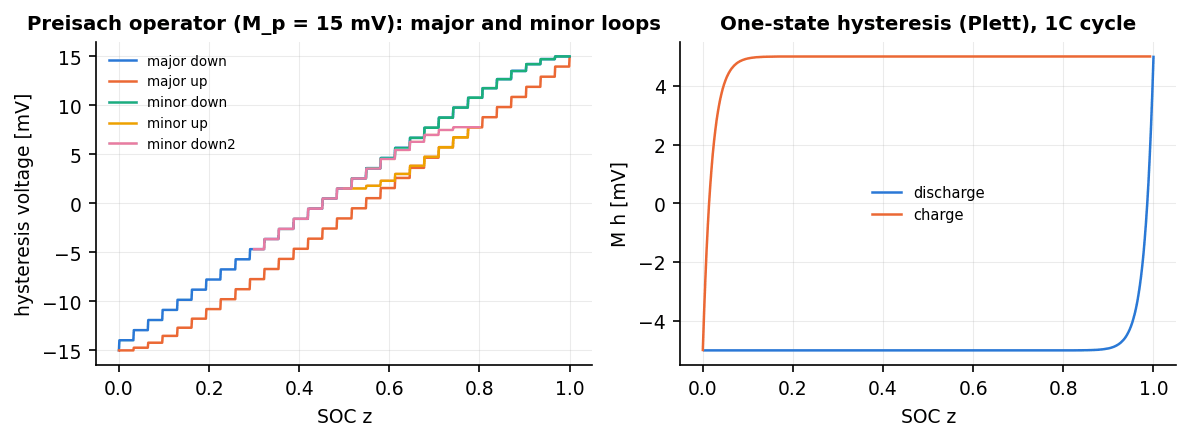
\includegraphics[width=\textwidth]{figures/model_hysteresis.png}
\caption{The two hysteresis models. Left: the 496-relay Preisach operator with
$M_p = \SI{15}{\milli\volt}$ and the Gaussian density \eqref{eq:ecm-mu}, showing the major
descending and ascending branches and a sequence of nested minor loops. The staircase is the
$L=32$ threshold quantisation (\num{0.032} SOC per step). Because $\mu$ is concentrated near the
diagonal $\alpha=\beta$, the operator behaves as a nearly affine, path-dependent function of SOC
with a loop opening of about \SI{3}{\milli\volt} and a full swing of $\pm\SI{15}{\milli\volt}$.
Right: the one-state model \eqref{eq:ecm-hyst-dt} over a 1C discharge followed by a 1C charge,
saturating at $\mp M = \mp\SI{5}{\milli\volt}$ within a few percent of SOC after each reversal.}
\label{fig:ecm-hyst}
\end{figure}

\begin{remark}[Loop orientation]\label{rem:ecm-orientation}
The two panels of \cref{fig:ecm-hyst} use opposite sign conventions and the reader should not be
misled. The Preisach operator is implemented with the classical relay convention
\eqref{eq:ecm-relay}, in which the \emph{descending} branch lies above the ascending one --- the
orientation of a magnetic $B$--$H$ loop. The one-state model uses the battery convention, in which
charging drives $h\to+1$ and the \emph{ascending} branch lies above. For the benchmark the
orientation is immaterial, because what the \code{preisach} scenario measures is the ability to
reject a rate-independent, path-dependent, SOC-correlated output disturbance that no estimator
model contains; the magnitude is what matters, and with $M_p=\SI{15}{\milli\volt}$ against the
estimator's $M=\SI{5}{\milli\volt}$ up to \SI{10}{\milli\volt} of it is irreducible --- about
\SI{1.2}{\percent} of SOC at a mid-range OCV slope.
\end{remark}

\section{The lumped thermal model}
\label{sec:ecm-thermal}

The plant carries a single thermal state, the cell temperature $T$, obeying the lumped energy
balance of Bernardi, Pawlikowski and Newman \cite{bernardi1985energy} with the lumped parameters
of Lin et~al.~\cite{lin2014thermal},
\begin{equation}
C_{\mathrm{th}}\frac{\mathrm{d}T}{\mathrm{d}t} =
 \underbrace{i\,\big(\ocv(\soc,T) - v\big)}_{\dot{q}_{\mathrm{irr}}}
 \;\underbrace{-\,i\,T\,\frac{\partial U}{\partial T}(\soc)}_{\dot{q}_{\mathrm{rev}}}
 \;-\;\frac{T - T_{\mathrm{amb}}}{R_{\mathrm{th}}} .
\label{eq:ecm-thermal}
\end{equation}

\paragraph{The irreversible term.} $\dot{q}_{\mathrm{irr}} = i\,(U-v)$ is the electrical power
dissipated in the overpotential. With the discharge-positive convention and
\eqref{eq:ecm-ct-out}, $U - v = v_1 + v_2 + R_0 i - Mh$, so
$\dot{q}_{\mathrm{irr}} = i(v_1+v_2+R_0 i) - iMh \ge 0$ for any realistic operating point: Joule
heating is sign-independent, as it must be.

\paragraph{The reversible term and its sign.} This is the term that is most often given the wrong
sign in the literature, so the derivation is worth spelling out. For a cell reaction transferring
$n$ electrons, $\Delta G = -nFU$ and, at constant pressure,
\begin{equation}
\Delta S = -\left.\frac{\partial(\Delta G)}{\partial T}\right|_p = nF\,\frac{\partial U}{\partial T}.
\label{eq:ecm-deltaS}
\end{equation}
On \emph{discharge} with $i>0$ the reaction proceeds at $\dot{\xi} = i/(nF)$ moles per second, so
the reversible heat \emph{absorbed} by the cell is
$T\Delta S\,\dot\xi = T\,nF(\partial U/\partial T)\,i/(nF) = i\,T\,\partial U/\partial T$, and the
reversible heat \emph{generated} is its negative,
\begin{equation}
\dot{q}_{\mathrm{rev}} = -\,i\,T\,\frac{\partial U}{\partial T}(\soc),
\label{eq:ecm-qrev}
\end{equation}
which is exactly the middle term of \eqref{eq:ecm-thermal} and exactly what the code computes.
For this cell $\partial U/\partial T<0$ everywhere, so \emph{discharge is entropically exothermic
and charge is entropically endothermic}, and reversing the current reverses the sign of
$\dot q_{\mathrm{rev}}$ while leaving $\dot q_{\mathrm{irr}}$ positive.

\paragraph{Magnitudes.} Per ampere, the reversible term contributes
$-T\,\partial U/\partial T = \SIrange{15}{60}{\milli\volt}$ of equivalent overpotential across the
SOC range at \SI{298}{\kelvin}. The irreversible term contributes
$v_1+v_2+R_0 i \approx \SI{26}{\milli\volt}$ per ampere at \SI{25}{\celsius} in steady state.
The entropic heat is therefore \emph{comparable to or larger than} the ohmic heat at low rates
and only a few percent of it during a 4.5C hover --- a strongly rate-dependent split that a
thermal model without \eqref{eq:ecm-qrev} would get badly wrong at cruise.

With $C_{\mathrm{th}} = \SI{70}{\joule\per\kelvin}$ (a \SI{70}{\gram} cell at
\SI{1000}{\joule\per\kilogram\per\kelvin}) and
$R_{\mathrm{th}} = \SI{3}{\kelvin\per\watt}$, the thermal time constant is
$C_{\mathrm{th}}R_{\mathrm{th}} = \SI{210}{\second}$ and the steady-state rise is
\SI{3}{\kelvin\per\watt} --- so the \SI{0.9}{\watt} of a 1.1C cruise settles at
$\approx\SI{2.7}{\kelvin}$ above ambient, while the \SI{8}{\watt} of a 4.5C hover would settle at
\SI{24}{\kelvin} but only reaches about \SI{7}{\kelvin} in the \SI{75}{\second} the hover lasts.
\eqref{eq:ecm-thermal} is integrated with an explicit Euler step, whose stability limit
$\dt < 2C_{\mathrm{th}}R_{\mathrm{th}} = \SI{420}{\second}$ is exceeded by a factor of
\num{4200} at $\dt=\SI{0.1}{\second}$.

\section{Arrhenius temperature dependence}
\label{sec:ecm-arrhenius}

All four impedance parameters are temperature scheduled by an Arrhenius law referred to
$T_{\mathrm{ref}}=\SI{298.15}{\kelvin}$ \cite[\S 2.10]{plett2015bms1,waag2013impedance},
\begin{equation}
p(T) = p(T_{\mathrm{ref}})\,
 \exp\!\left[\frac{E_{a,p}}{R_g}\left(\frac{1}{T}-\frac{1}{T_{\mathrm{ref}}}\right)\right],
\qquad p \in \{R_0, R_1, R_2, \tau_1, \tau_2\},
\label{eq:ecm-arrhenius}
\end{equation}
with $R_g = \SI{8.3145}{\joule\per\mole\per\kelvin}$. Note the sign: for $T<T_{\mathrm{ref}}$ the
bracket is positive, so \emph{resistances and time constants both grow as the cell cools} --- the
process being activated is charge transfer and solid-state diffusion, whose rates fall with
temperature. (The single-particle plant of \cref{ch:spm} uses the reciprocal convention for
$D$ and $j_0$, which are transport coefficients and therefore \emph{fall} when cold; the physics
is the same.)

\begin{figure}[H]\centering
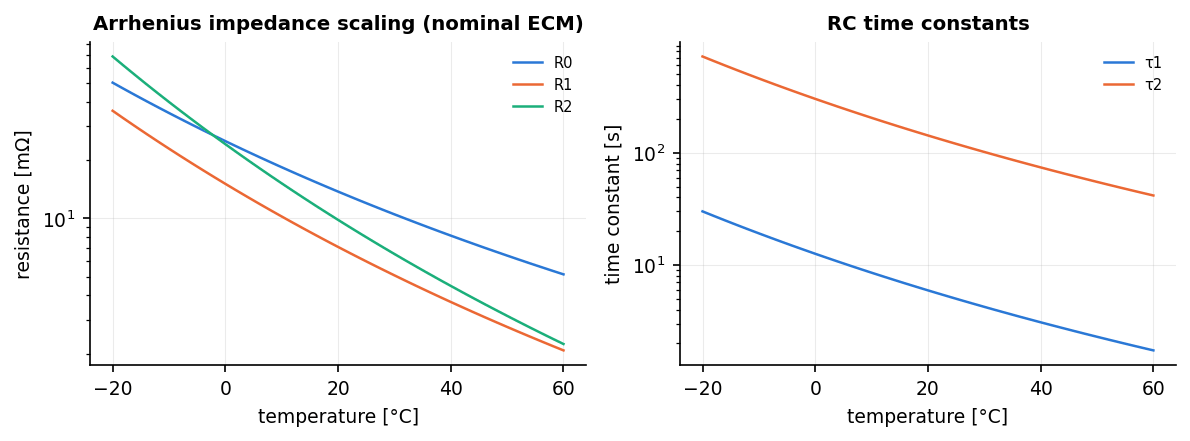
\includegraphics[width=\textwidth]{figures/model_arrhenius.png}
\caption{Arrhenius scheduling \eqref{eq:ecm-arrhenius} of the nominal parameter set over
$\SIrange{-20}{60}{\celsius}$. Left: the three resistances, on a logarithmic scale, so that
\eqref{eq:ecm-arrhenius} plots as a nearly straight line in $1/T$; the different activation
energies make the curves cross near $\SI{-2}{\celsius}$, where $R_2$ overtakes $R_0$ as the
dominant impedance. Right: the two time constants, which grow from \SI{1.7}{\second} and
\SI{42}{\second} at \SI{60}{\celsius} to \SI{30}{\second} and \SI{721}{\second} at
\SI{-20}{\celsius}.}
\label{fig:ecm-arrhenius}
\end{figure}

\cref{tab:ecm-arrhenius} lists the scheduled values at the three benchmark temperatures. The
range is the reason the \code{cold} scenario is hard: at $\SI{-10}{\celsius}$ the ohmic drop at a
4.5C hover is \SI{790}{\milli\volt} instead of \SI{270}{\milli\volt}, the slow time constant is
\SI{459}{\second} --- longer than the entire climb segment --- and any error in $R_0$ is
amplified threefold.

\begin{table}[H]\centering
\caption{Nominal ECM parameters under the Arrhenius schedule \eqref{eq:ecm-arrhenius}.}
\label{tab:ecm-arrhenius}
\begin{tabular}{lccccc}\toprule
$T$ & $R_0$ [\si{\milli\ohm}] & $R_1$ [\si{\milli\ohm}] & $R_2$ [\si{\milli\ohm}]
    & $\tau_1$ [\si{\second}] & $\tau_2$ [\si{\second}] \\ \midrule
\SI{-10}{\celsius} & 35.1 & 22.9 & 40.0 & 19.1 & 458.9 \\
\SI{25}{\celsius}  & 12.0 &  6.0 &  8.0 &  5.0 & 120.0 \\
\SI{45}{\celsius}  &  7.2 &  3.2 &  3.7 &  2.6 &  63.7 \\
\bottomrule\end{tabular}
\end{table}

\section{Ageing}
\label{sec:ecm-aging}

The plant loses capacity and gains resistance as it is used and as it sits. The library follows
the structural form of Wang et~al.~\cite{wang2011cyclelife} --- an Arrhenius factor multiplying a
power law in ampere-hour throughput --- with an added calendar term of the type used by
Schmalstieg et~al.~\cite{schmalstieg2014aging}.

\subsection{Cycle ageing}
Wang's law for the lost capacity fraction after a throughput $A_h$ (\si{\ampere\hour}) at
constant temperature is
\begin{equation}
Q_{\mathrm{loss}} = B\,\exp\!\left(-\frac{E_a}{R_g T}\right) A_h^{\,\zeta},
\qquad \zeta = 0.55, \quad E_a = \SI{31700}{\joule\per\mole}.
\label{eq:ecm-wang}
\end{equation}
Because the temperature varies along a mission, the library integrates the \emph{rate} form
obtained by differentiating \eqref{eq:ecm-wang} at fixed $T$,
\begin{equation}
\mathrm{d}Q_{\mathrm{loss}} = B\,\exp\!\left(-\frac{E_a}{R_g T}\right)\zeta\,A_h^{\,\zeta-1}\,
 \mathrm{d}A_h, \qquad \mathrm{d}A_h = \frac{|i|\,\dt}{3600},
\label{eq:ecm-wang-rate}
\end{equation}
which reduces to \eqref{eq:ecm-wang} at constant temperature and gives a path-dependent
(and physically more plausible) answer otherwise.

\subsection{Calendar ageing and resistance growth}
Storage adds a square-root-of-time term evaluated at the ambient temperature, applied by the
benchmark between flights,
\begin{equation}
\Delta Q_{\mathrm{loss}}^{\mathrm{cal}} = A_{\mathrm{cal}}
 \exp\!\left(-\frac{E_{a,\mathrm{cal}}}{R_g T_{\mathrm{amb}}}\right)
 \left(\sqrt{t_1} - \sqrt{t_0}\right),
\label{eq:ecm-calendar}
\end{equation}
with $t$ in days. Resistance growth is tied to capacity loss by a single gain,
\begin{equation}
R_0^{\mathrm{aged}}(T) = R_0(T)\left(1 + k_R\,Q_{\mathrm{loss}}\right), \qquad k_R = 2.5 .
\label{eq:ecm-Rgrowth}
\end{equation}

\begin{figure}[H]\centering
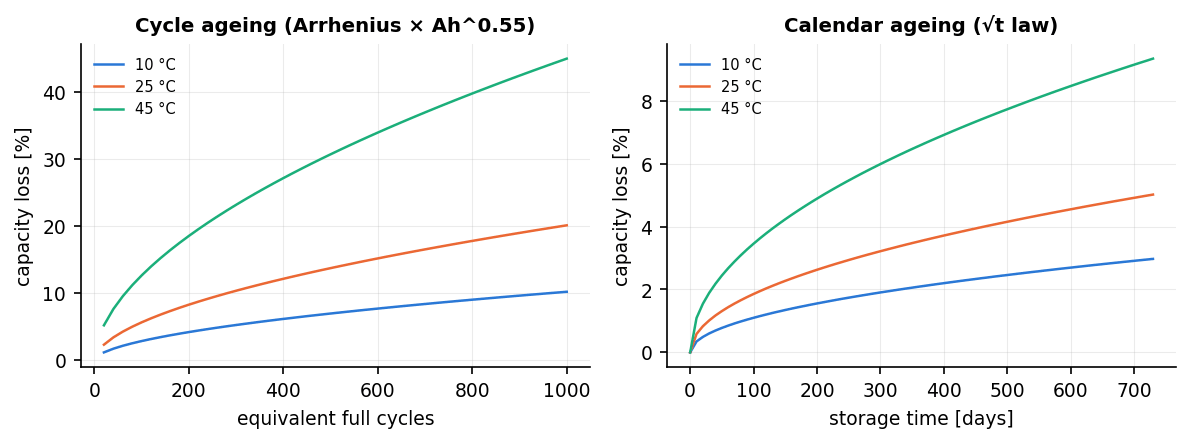
\includegraphics[width=\textwidth]{figures/model_aging.png}
\caption{Ageing of the ECM plant. Left: capacity loss under 1C full cycles from
\eqref{eq:ecm-wang-rate} at three temperatures; the curves reach \SI{10.2}{\percent},
\SI{20.1}{\percent} and \SI{44.9}{\percent} after 1000 equivalent full cycles at
\SI{10}{\celsius}, \SI{25}{\celsius} and \SI{45}{\celsius}. Right: calendar ageing from
\eqref{eq:ecm-calendar}, reaching \SI{3.0}{\percent}, \SI{5.0}{\percent} and
\SI{9.3}{\percent} after two years of storage at the same three temperatures.}
\label{fig:ecm-aging}
\end{figure}

\begin{remark}[Status of the ageing coefficients]\label{rem:ecm-aging}
Only the \emph{structure} of \eqref{eq:ecm-wang}--\eqref{eq:ecm-calendar} and the exponents
$\zeta = 0.55$, $E_a = \SI{31700}{\joule\per\mole}$ come from the literature. The prefactors are
representative values chosen to calibrate the plant to two round numbers that are conventional
end-of-life criteria: $B = \num{454}$ (in units of $\si{\ampere\hour}^{-\zeta}$) gives exactly
\SI{20}{\percent} capacity loss after 1000 equivalent full cycles (\SI{10000}{\ampere\hour} of
throughput for a \SI{5}{\ampere\hour} cell) at \SI{25}{\celsius}, and
$A_{\mathrm{cal}} = 36.4$ with $E_{a,\mathrm{cal}} = \SI{24500}{\joule\per\mole}$ gives exactly
\SI{5}{\percent} loss after two years of storage at \SI{25}{\celsius}. They are \emph{not} fitted
to measurements of an NMC811 cell and no claim is made that they predict one; they exist so that
the multi-flight state-of-health benchmark of Part~XIII has a smooth, temperature-sensitive,
monotone truth to track.
\end{remark}

\section{The estimator-side model}
\label{sec:ecm-estimator}

Everything above describes the plant. The model handed to every estimator, \code{EcmModel}, is
deliberately poorer and is what a real BMS would run.

\subsection{State, input, output}
\begin{equation}
\vx = \begin{bmatrix}\soc & v_1 & v_2 & h\end{bmatrix}^\T \in \real^4, \qquad
\vu = \begin{bmatrix}i & T\end{bmatrix}^\T\in\real^2, \qquad
y = v \in \real,
\label{eq:ecm-state}
\end{equation}
so $n_x=4$, $n_u=2$, $n_y=1$. The current $i$ is a true input and the temperature $T$ a
scheduling variable in the sense of \cref{rem:prelim-sched}. The dynamics are
\eqref{eq:ecm-zoh}, \eqref{eq:ecm-coulomb} and \eqref{eq:ecm-hyst-dt} collected into
\begin{equation}
f(\vx,\vu) = \begin{bmatrix}
 \soc - \dfrac{\eta(i)\dt}{3600\,Q}\,i \\[2mm]
 a_1(T)\,v_1 + R_1(T)\big(1-a_1(T)\big) i \\[2mm]
 a_2(T)\,v_2 + R_2(T)\big(1-a_2(T)\big) i \\[2mm]
 a_h(i)\,h + \big(a_h(i)-1\big)\sgn(i)
\end{bmatrix},
\qquad
h(\vx,\vu) = \ocv(\soc,T) + M h - v_1 - v_2 - R_0(T)\,i .
\label{eq:ecm-fh}
\end{equation}

\subsection{Jacobians in closed form}
All three Jacobians are available analytically, which is why the cell benchmark runs seventy
estimators over twelve scenarios in minutes:
\begin{align}
\mF(\vu) &= \diag\!\big(1,\ a_1(T),\ a_2(T),\ a_h(i)\big),
\label{eq:ecm-F}\\[1mm]
\mB(\vx,\vu) &= \begin{bmatrix}
 -\dfrac{\eta(i)\dt}{3600\,Q} & 0\\[2mm]
 R_1(T)\big(1-a_1(T)\big) & 0\\[2mm]
 R_2(T)\big(1-a_2(T)\big) & 0\\[2mm]
 \dfrac{\partial a_h}{\partial i}\big(h + \sgn(i)\big) & 0
\end{bmatrix},
\quad
\frac{\partial a_h}{\partial i} = -\sgn(i)\,\frac{\eta(i)\gamma\dt}{3600\,Q}\,a_h(i),
\label{eq:ecm-B}\\[1mm]
\mH(\vx,\vu) &= \begin{bmatrix}
 \dfrac{\partial\ocv}{\partial\soc}(\soc,T) & -1 & -1 & M
\end{bmatrix},
\qquad
\frac{\partial h}{\partial i} = -R_0(T).
\label{eq:ecm-H}
\end{align}

Three structural features of \eqref{eq:ecm-F}--\eqref{eq:ecm-H} recur throughout the report.
First, $\mF$ is \emph{diagonal}: the four states are dynamically decoupled and are coupled only
through the scalar measurement. Every correlation in $\mP$ is therefore created by the update,
never by the prediction. Second, the SOC row of $\mF$ is exactly $1$ --- a pure integrator with
no forgetting, so an SOC error persists until a measurement removes it. Third, the second column
of $\mB$ is identically zero: the model neglects $\partial f/\partial T$. This is justified
numerically --- the largest entry it would contain,
$\partial v_1^+/\partial T \approx \SI{-2e-5}{\volt\per\kelvin}$, produces
\SI{4e-6}{\volt} of spread at $\sigma_T = \SI{0.2}{\kelvin}$, some \num{25} times below the
process-noise floor --- and it is stated here because it is an approximation, not an identity.

\subsection{Process and measurement noise}
The covariances are built from the sensor data sheet rather than tuned:
\begin{align}
\mQ(\vx,\vu) &= \bm{b}\,\bm{b}^\T\sigma_i^2 + \diag\!\big(q_{\mathrm{floor}}^2\big),
 \qquad \bm{b} = \mB(\vx,\vu)\,\bm{e}_1 = \frac{\partial f}{\partial i},
\label{eq:ecm-Q}\\
\mR(\vu) &= \sigma_v^2 + \big(R_0(T)\,\sigma_i\big)^2 .
\label{eq:ecm-R}
\end{align}
The construction of \eqref{eq:ecm-Q} is the important one: current-sensor noise is not an
independent disturbance on each state but enters through the same channel as the current itself,
so its covariance contribution is the rank-one matrix $\bm{b}\bm{b}^\T\sigma_i^2$. The diagonal
floor $q_{\mathrm{floor}} = (\num{1e-5},\ \num{1e-4},\ \num{1e-4},\ \num{1e-3})$ --- in SOC, volts,
volts and dimensionless units respectively --- keeps $\mQ\succ0$ when the current is zero, which
would otherwise make $\bm{b}\bm{b}^\T$ singular and freeze the filter during a rest. Similarly,
\eqref{eq:ecm-R} adds to the voltage-sensor variance the feed-through of current noise through
the ohmic drop, $(\partial h/\partial i)^2\sigma_i^2$. With
$\sigma_v = \SI{2}{\milli\volt}$ and $\sigma_i = \SI{50}{\milli\ampere}$ the second term
contributes \SI{0.6}{\milli\volt} at \SI{25}{\celsius} and \SI{1.8}{\milli\volt} when cold.

\begin{remark}[An omitted term in $\mR$]\label{rem:ecm-Romission}
\eqref{eq:ecm-R} does not include the feed-through of \emph{temperature}-sensor noise,
$(i\,\partial R_0/\partial T\,\sigma_T)^2$. Since
$\partial R_0/\partial T = -R_0 E_a/(R_g T^2) = \SI{-3.2e-4}{\ohm\per\kelvin}$ at
\SI{25}{\celsius}, this term is \SI{0.3}{\milli\volt} at 1C --- negligible against
$\sigma_v$ --- but \SI{1.5}{\milli\volt} at the 4.5C hover, where it is no longer negligible.
The benchmark keeps the omission deliberately: it is a small, load-correlated modelling error of
exactly the kind that adaptive and robust filters are supposed to absorb.
\end{remark}

\subsection{The OCV lookup table}
\label{sec:ecm-lut}
The plant evaluates \eqref{eq:ecm-ocv} in closed form. The estimator instead carries what a BMS
stores in flash: a uniform table of $N=241$ points over $\soc\in[-0.1,1.1]$, hence a grid spacing
of $\Delta\soc = 0.005$, with linear interpolation inside and linear extrapolation outside, plus
the analytic entropic correction \eqref{eq:ecm-ocvT}:
\begin{equation}
\widehat{\ocv}(\soc,T) = v_j + d_j\,(\soc - \soc_j) + (T-T_{\mathrm{ref}})\frac{\partial U}{\partial T}(\soc),
\qquad
\frac{\partial\widehat{\ocv}}{\partial\soc} = d_j + (T-T_{\mathrm{ref}})
 \frac{\partial^2 U}{\partial T\,\partial\soc},
\label{eq:ecm-lut}
\end{equation}
with $j = \lfloor(\soc-\soc_{\mathrm{lo}})/\Delta\soc\rfloor$ and $d_j$ the segment slope. The
interpolation error is \SI{0.164}{\milli\volt} at worst over $\soc\in[0.05,1]$ and
\SI{0.013}{\milli\volt} in root-mean-square over $\soc\in[0.2,0.95]$: an order of magnitude below
the sensor noise and therefore irrelevant as a voltage error. The \emph{slope} error is a
different matter --- up to \SI{0.13}{\volt} near $\soc=0.12$, where the curve bends sharply within
one table segment --- which against the true slope of \SI{2.22}{\volt} there is a
\SI{6}{\percent} error in the measurement Jacobian.
The lookup table also makes $\partial\widehat{\ocv}/\partial\soc$ piecewise constant and therefore
discontinuous at the knots, which is invisible to an EKF but does perturb the numerical Jacobians
of derivative-free filters if their sigma points straddle a knot.

\subsection{Constraints, parameters and initialisation}
The feasible set is a box,
$\mathcal{X} = \{\soc\in[-0.05,\,1.05],\ h\in[-1,\,1]\}$, and the projection onto it is applied
after the update by every filter that declares \code{apply\_constraints}; the small slack outside
$[0,1]$ prevents the constraint from biasing the estimate at the ends of the range
\cite{simon2010constraints}. For joint and dual estimation the model exposes
$\vtheta = [Q,\ R_0]^\T$ with the positivity guards $Q\ge\SI{0.5}{\ampere\hour}$ and
$R_0\ge\SI{0.1}{\milli\ohm}$. The default initialisation is
\begin{equation}
\xhat_0 = \begin{bmatrix}\soc_0 & 0 & 0 & 0\end{bmatrix}^\T,\qquad
\mP_0 = \diag\!\left(\sigma_{\soc,0}^2,\ (\SI{2}{\milli\volt})^2,\ (\SI{5}{\milli\volt})^2,\
 0.5^2\right),
\label{eq:ecm-init}
\end{equation}
with $\sigma_{\soc,0}=0.1$ --- a deliberately loose prior, because it is the combination of a
loose prior with a curved $\ocv$ that separates the estimators.

\section{Observability of the four-state model}
\label{sec:ecm-obs}

Apply \eqref{eq:prelim-obsmat} to \eqref{eq:ecm-F}--\eqref{eq:ecm-H} with the Jacobians frozen at
an operating point. Writing $c_\soc = \partial\ocv/\partial\soc$ and
$\bm\lambda = (1,\,a_1,\,a_2,\,a_h)$, row $j$ of the observability matrix is
$\mH\mF^{j} = \left[\,c_\soc,\ -a_1^{\,j},\ -a_2^{\,j},\ M a_h^{\,j}\,\right]$, so that
\begin{equation}
\mathcal{O}_4 = \bm{V}\,\diag\!\left(c_\soc,\,-1,\,-1,\,M\right),
\qquad V_{jk} = \lambda_k^{\,j},\ \ j,k = 0,\dots,3 .
\label{eq:ecm-Ostruct}
\end{equation}
$\bm{V}$ is a Vandermonde matrix, so the determinant is available in closed form.

\begin{proposition}[Rank condition]\label{prop:ecm-rank}
$\det\mathcal{O}_4 = c_\soc\,M\prod_{k<l}(\lambda_l-\lambda_k)$. The linearised four-state model
is observable if and only if $c_\soc\neq 0$, $M\neq 0$, and the four modes
$1, a_1, a_2, a_h$ are pairwise distinct.
\end{proposition}

Each of the three conditions has a physical meaning and each is violated somewhere in the
benchmark.
\begin{itemize}[nosep,leftmargin=*]
\item $c_\soc\ne 0$ is the OCV-slope condition of \cref{sec:prelim-ocvslope}. It never fails
  exactly for this chemistry but comes within a factor of six of doing so at $\soc\approx0.90$.
\item $M\ne 0$ is needed because $h$ enters the output only through $M$. The parameter set
  identified against the single-particle plant in \cref{ch:spm} sets $M=0$, because the SPM has
  no hysteresis; there the four-state model is structurally unobservable and the correct model is
  the three-state one, $[\soc,v_1,v_2]$, which is observable with a condition number smaller by
  six orders of magnitude.
\item $a_h = \exp(-\gamma|\Delta\soc|)\to 1$ as $i\to0$. During a rest the hysteresis mode
  coincides with the SOC mode and observability is lost --- correctly, since a resting cell
  reveals nothing about the sign of its last current beyond what $h$ already encodes.
\end{itemize}

The rank test is, however, far too crude; the singular values are the informative object.
\cref{tab:ecm-obs} lists them for the four-sample matrix $\mathcal{O}_4$ and for longer horizons.

\begin{table}[H]\centering
\caption{Singular values of the linearised observability matrix $\mathcal{O}_N$ of the cell
model, $\dt=\SI{0.1}{\second}$, 1C discharge, nominal parameters. The last column is
$\sigma_{\max}/\sigma_{\min}$, the degree of unobservability of \cref{sec:prelim-obs}.}
\label{tab:ecm-obs}
\small
\begin{tabular}{llcccc c}\toprule
Operating point & $N$ & $\sigma_1$ & $\sigma_2$ & $\sigma_3$ & $\sigma_4$ & cond \\ \midrule
$\soc=0.7$, \SI{25}{\celsius} ($c_\soc=\num{0.93}$) & 4 & \num{3.35} & \num{3.5e-2} & \num{1.1e-5} & \num{1.6e-11} & \num{2.1e11}\\
$\soc=0.90$, \SI{25}{\celsius} ($c_\soc=\num{0.196}$) & 4 & \num{2.81} & \num{3.0e-2} & \num{3.2e-6} & \num{1.6e-11} & \num{1.8e11}\\
$\soc=0.7$, \SI{-10}{\celsius} & 4 & \num{3.38} & \num{9.2e-3} & \num{7.6e-7} & \num{7.0e-12} & \num{4.8e11}\\[1mm]
$\soc=0.7$, \SI{25}{\celsius} & 100 (\SI{10}{\second}) & \num{14.1} & \num{2.27} & \num{3.9e-2} & \num{2.1e-6} & \num{6.8e6}\\
$\soc=0.7$, \SI{25}{\celsius} & 1200 (\SI{120}{\second}) & \num{39.2} & \num{6.14} & \num{3.41} & \num{2.4e-3} & \num{1.6e4}\\
$\soc=0.7$, \SI{25}{\celsius} & 6000 (\SI{600}{\second}) & \num{73.8} & \num{18.7} & \num{4.56} & \num{1.6e-2} & \num{4.5e3}\\
\bottomrule\end{tabular}
\end{table}

Three readings of \cref{tab:ecm-obs} carry through the whole report.

\paragraph{Observability is a function of the horizon, not of the model.} The minimal
four-sample test gives a condition number of $10^{11}$: over \SI{0.4}{\second} the four modes are
numerically indistinguishable and the problem is, for practical purposes, unobservable. Extending
the window to \SI{600}{\second} improves the conditioning by eight orders of magnitude. This is
the quantitative reason why filters converge slowly after a reset even though the pair
$(\mF,\mH)$ passes a rank test at every sample, and why the moving-horizon methods of Part~IX,
which use a window explicitly, behave differently from the recursive ones.

\paragraph{A flat OCV costs a factor of three, not a rank.} Moving from $\soc=0.7$ to the
plateau at $\soc=0.90$ reduces $\sigma_3$ from \num{1.1e-5} to \num{3.2e-6}, a factor of
\num{3.5}, without changing the rank. The consequence is an error \emph{gain}, not a failure:
\begin{equation}
\delta\soc \;\approx\; \frac{\delta v}{\partial\ocv/\partial\soc},
\label{eq:ecm-errgain}
\end{equation}
so any unmodelled voltage error $\delta v$ is converted into an SOC error at a rate set by the
inverse slope. At $\soc=0.90$ the gain is $1/\num{0.196} = \SI{5.1}{\per\volt}$: a
\SI{4}{\milli\volt} structured model error --- exactly the residual of the ECM fitted to the
single-particle plant in \cref{ch:spm} --- is worth \SI{2.0}{\percent} of SOC, and the
\SI{10}{\milli\volt} of unmodelled Preisach hysteresis of \cref{rem:ecm-orientation} is worth
\SI{5}{\percent}. No amount of filtering removes a bias that the model itself does not contain.

\paragraph{The slow branch is confusable with the SOC.} The worst-conditioned direction is not
$\soc$ alone but the $(\soc, v_2)$ combination, because the SOC integrator has mode
$\lambda=1$ and the slow branch has $a_2 = 0.999167$. The angle between the corresponding columns
of $\mathcal{O}_N$ over a window of length $T$ is
\begin{equation}
\cos\theta(T) = \frac{\sum_{j} a_2^{\,j}}{\sqrt{N}\ \sqrt{\sum_j a_2^{2j}}},
\qquad N = T/\dt,
\label{eq:ecm-angle}
\end{equation}
which is listed in \cref{tab:ecm-angle}. Over ten seconds the two directions are
\SI{1.4}{\degree} apart: an SOC error and a slow-polarisation error produce voltage signatures
that differ by about one part in \num{400}, far below the \SI{2}{\milli\volt} noise floor. This
is why a load step is followed by a slow SOC transient in nearly every trace in Part~XIII, and
why the effect is much worse for the SPM-fitted parameter set ($\tau_2 = \SI{556}{\second}$) than
for the nominal one ($\tau_2 = \SI{120}{\second}$).

\begin{table}[H]\centering
\caption{Angle \eqref{eq:ecm-angle} between the $\soc$ and $v_2$ columns of the observability
matrix as a function of the observation window.}
\label{tab:ecm-angle}
\begin{tabular}{lcccccc}\toprule
window $T$ & \SI{1}{\second} & \SI{10}{\second} & \SI{60}{\second} & \SI{300}{\second} & \SI{600}{\second} & \SI{1800}{\second}\\ \midrule
$\theta$, $\tau_2=\SI{120}{\second}$ (nominal)  & \ang{0.14} & \ang{1.38} & \ang{8.20} & \ang{34.5} & \ang{51.1} & \ang{68.6}\\
$\theta$, $\tau_2=\SI{556}{\second}$ (SPM fit)  & \ang{0.03} & \ang{0.30} & \ang{1.78} & \ang{8.84} & \ang{17.2} & \ang{40.9}\\
\bottomrule\end{tabular}
\end{table}

Finally, a structural non-observability that no conditioning number reveals: a \emph{current
sensor bias} added to the state would make the augmented pair unobservable from a single voltage
measurement, because bias and SOC enter the output through the same integrator channel. Zhao,
Duncan and Howey \cite{zhao2017observability} prove this and identify the excitation that
restores observability; Lin \cite{lin2018sensorbias} gives the resulting steady-state SOC error
as an explicit function of the bias and the OCV slope. This is the theoretical content of the
\code{current\_bias} scenario and the reason it is the scenario on which the unknown-input and
disturbance observers of Part~VI earn their place.

\section{Parameters of the nominal cell}
\label{sec:ecm-params}

\cref{tab:ecm-chen,tab:ecm-cellparams} list every constant of the plant with its provenance. The
parameter set identified against the single-particle plant, which is what the SPM benchmark gives
the estimators, is reported in \cref{ch:spm}.

\begin{table}[H]\centering
\caption{Electrode data used to construct the OCV, from Chen et~al.~\cite{chen2020parameterization}
as distributed in the PyBaMM \texttt{Chen2020} parameter set (LG~M50, NMC811/graphite,
21700 format).}
\label{tab:ecm-chen}
\begin{tabular}{llcc}\toprule
Quantity & Symbol & Negative (graphite) & Positive (NMC811) \\ \midrule
Electrode area & $A$ & \multicolumn{2}{c}{\SI{0.1027}{\square\metre}} \\
Coating thickness & $L_k$ & \SI{85.2}{\micro\metre} & \SI{75.6}{\micro\metre}\\
Active volume fraction & $\varepsilon_k$ & \num{0.75} & \num{0.665}\\
Particle radius & $R_k$ & \SI{5.86}{\micro\metre} & \SI{5.22}{\micro\metre}\\
Maximum concentration & $c_{\max,k}$ & \SI{33133}{\mole\per\cubic\metre} & \SI{63104}{\mole\per\cubic\metre}\\
Charge per unit stoichiometry & $q_k$ & \SI{5.83}{\ampere\hour} & \SI{8.73}{\ampere\hour}\\
Stoichiometry at $\soc=1$ & $x_{100}, y_{100}$ & \num{0.9014} & \num{0.2700}\\
Stoichiometry at $\soc=0$ & $x_{0}, y_{0}$ & \num{0.04342} & \num{0.84259}\\
Stoichiometry span & $\Delta x, \Delta y$ & \num{0.85798} & \num{0.57259}\\
\bottomrule\end{tabular}
\end{table}

\begin{table}[H]\centering
\caption{Nominal equivalent-circuit, thermal and ageing parameters
(\code{CellParams::nominal()}). ``Representative'' means the value is of the right order for this
cell class but is not a fit to measured data for it.}
\label{tab:ecm-cellparams}
\small
\begin{tabular}{llll}\toprule
Parameter & Symbol & Value & Source \\ \midrule
Nominal capacity & $Q$ & \SI{5.0}{\ampere\hour} & \cite{chen2020parameterization}\\
Coulombic efficiency (charge) & $\eta_c$ & \num{0.995} & \cite{ng2009coulomb,smith2010coulombic}\\
Ohmic resistance & $R_0$ & \SI{12.0}{\milli\ohm} & representative\\
Fast branch & $R_1,\tau_1$ & \SI{6.0}{\milli\ohm}, \SI{5}{\second} & representative\\
Slow branch & $R_2,\tau_2$ & \SI{8.0}{\milli\ohm}, \SI{120}{\second} & representative\\
Hysteresis magnitude & $M$ & \SI{5}{\milli\volt} & \cite{plett2004ekf1,plett2015bms1}\\
Hysteresis rate & $\gamma$ & \num{50} & \cite{plett2015bms1}\\
Preisach half-width (plant) & $M_p$ & \SI{15}{\milli\volt} & \cite{baronti2014hysteresis}\\
Activation energy, $R_0$ & $E_{a,R_0}$ & \SI{20}{\kilo\joule\per\mole} & \cite{plett2015bms1,waag2013impedance}\\
Activation energy, $R_1$ & $E_{a,R_1}$ & \SI{25}{\kilo\joule\per\mole} & \cite{plett2015bms1}\\
Activation energy, $R_2$ & $E_{a,R_2}$ & \SI{30}{\kilo\joule\per\mole} & \cite{plett2015bms1}\\
Activation energy, $\tau_j$ & $E_{a,\tau}$ & \SI{25}{\kilo\joule\per\mole} & \cite{plett2015bms1}\\
Reference temperature & $T_{\mathrm{ref}}$ & \SI{298.15}{\kelvin} & ---\\
Lumped heat capacity & $C_{\mathrm{th}}$ & \SI{70}{\joule\per\kelvin} & \cite{lin2014thermal}\\
Cell-to-ambient resistance & $R_{\mathrm{th}}$ & \SI{3}{\kelvin\per\watt} & \cite{lin2014thermal}\\
Cycle-ageing prefactor & $B$ & \num{454} & representative (\cref{rem:ecm-aging})\\
Cycle-ageing activation energy & $E_a$ & \SI{31.7}{\kilo\joule\per\mole} & \cite{wang2011cyclelife}\\
Cycle-ageing exponent & $\zeta$ & \num{0.55} & \cite{wang2011cyclelife}\\
Calendar prefactor & $A_{\mathrm{cal}}$ & \num{36.4} & representative (\cref{rem:ecm-aging})\\
Calendar activation energy & $E_{a,\mathrm{cal}}$ & \SI{24.5}{\kilo\joule\per\mole} & \cite{schmalstieg2014aging}\\
Resistance-growth gain & $k_R$ & \num{2.5} & \cite{schmalstieg2014aging}\\[1mm]
Sample period & $\dt$ & \SI{0.1}{\second} & ---\\
Voltage-sensor noise & $\sigma_v$ & \SI{2}{\milli\volt} (\SI{1}{\milli\volt} quantisation) & ---\\
Current-sensor noise & $\sigma_i$ & \SI{50}{\milli\ampere} (\SI{10}{\milli\ampere} quantisation) & ---\\
Temperature-sensor noise & $\sigma_T$ & \SI{0.2}{\kelvin} & ---\\
\bottomrule\end{tabular}
\end{table}

\section{Plant versus estimator: the deliberate mismatches}
\label{sec:ecm-mismatch}

A benchmark in which the estimator's model equals the plant measures numerical hygiene and
nothing else. The gaps listed in \cref{tab:ecm-mismatch} are therefore the experiment. They are
chosen to be of the kinds that a real BMS faces --- a table instead of a function, an unmodelled
thermal state, a structurally different hysteresis, a drifting capacity, a biased current sensor
--- and each is individually small enough to be plausible and large enough to separate the
estimators.

\begin{table}[H]\centering
\caption{Differences between the truth plant (\code{EcmPlant}) and the model given to the
estimators (\code{EcmModel}), with the magnitude of each and the benchmark scenario that
exercises it.}
\label{tab:ecm-mismatch}
\begin{tabular}{p{31mm}p{37mm}p{37mm}p{28mm}}\toprule
Mechanism & Plant & Estimator & Magnitude / scenario \\ \midrule
Open-circuit voltage & closed-form electrode potentials \eqref{eq:ecm-ocv} &
 241-point table \eqref{eq:ecm-lut} &
 $\le\SI{0.16}{\milli\volt}$; slope error up to \SI{0.13}{\volt}; all scenarios \\
Thermal state & lumped ODE \eqref{eq:ecm-thermal} with reversible heat &
 none; measured $T$ used as a scheduling input &
 self-heating up to \SI{7}{\kelvin} in hover; \code{cold}, \code{hot} \\
Hysteresis & one-state or 496-relay Preisach, $M_p=\SI{15}{\milli\volt}$ &
 one-state only, $M=\SI{5}{\milli\volt}$ &
 up to \SI{10}{\milli\volt} irreducible; \code{preisach} \\
Ageing & continuous capacity fade \eqref{eq:ecm-wang-rate} and resistance growth
 \eqref{eq:ecm-Rgrowth} & fixed $Q$, $R_0$ unless an SOH method &
 \SI{15}{\percent} capacity loss, $R_0\times\num{1.375}$; \code{aged\_cell} \\
Impedance parameters & true Arrhenius-scaled values & optionally scaled: $R_0\times\num{0.7}$,
 $R_1\times\num{1.3}$, $\tau_2\times\num{1.5}$ & \code{param\_mismatch} \\
Current sensor & --- & gain $g$, bias $b$, noise, \SI{10}{\milli\ampere} quantisation; only the
 white part appears in $\mQ$ & $g=\num{1.02}$, $b=\SI{0.25}{\ampere}$; \code{current\_bias} \\
Voltage sensor & --- & noise, \SI{1}{\milli\volt} quantisation, outliers, stuck-at dropout;
 only the white part appears in $\mR$ &
 \SI{50}{\milli\volt} outliers at \SI{5}{\percent}; \SI{15}{\second} dropout;
 \code{outliers}, \code{noise\_step}, \code{sensor\_dropout} \\
Temperature sensor & --- & noise; feed-through omitted from $\mR$
 (\cref{rem:ecm-Romission}) & \SI{1.5}{\milli\volt} at 4.5C \\
\bottomrule\end{tabular}
\end{table}

The \code{combined} scenario switches several of these on at once --- a \SI{-25}{\percent}
initial SOC error, a \SI{0.15}{\ampere} current bias with a \SI{2}{\percent} gain error,
\SI{10}{\percent} capacity loss and a \SI{0}{\celsius} ambient --- and it is the scenario on which
the plain EKF fails and the moment-matching, robust and constrained filters do not. That result,
and its explanation in terms of \cref{as:prelim-lin} and \eqref{eq:ecm-errgain}, is the subject of
Part~XIII.

\section{Summary}

The cell model of this chapter is an integrator with no forgetting, observed through a single
nonlinear map whose derivative --- the OCV slope of \cref{fig:ecm-ocv} --- ranges over a factor of
six and reaches its minimum precisely where the missions begin. Around that core sit three
relaxation states (two RC branches and a hysteresis variable), an Arrhenius schedule that
multiplies every impedance by five between \SI{45}{\celsius} and \SI{-10}{\celsius}, a thermal
state whose reversible heat is comparable to its irreversible heat at low rates, and an ageing
law that moves the capacity out from under the definition of SOC itself. The estimator is given
four of those states, a tabulated OCV, and a measured temperature. \cref{ch:spm} replaces the
plant by an electrochemical model that shares none of the equivalent circuit's structure, and
measures what the resulting structured model error does to seventy estimators.
